\documentclass[11pt,letterpaper]{article}

% Build steps (from this folder):
% 1) pdflatex Module4.tex
% 2) makeglossaries Module4
% 3) pdflatex Module4.tex
% 4) pdflatex Module4.tex

% ── Packages ──────────────────────────────────────────────────
\usepackage[margin=1in]{geometry}
\usepackage{titlesec}
\usepackage{enumitem}
\usepackage{booktabs}
\usepackage{tabularx}
\usepackage{graphicx}
\usepackage{xcolor}
\usepackage{hyperref}
\usepackage{fancyhdr}
\usepackage{amsmath}
\usepackage{amssymb}
\usepackage{tcolorbox}
\usepackage{multicol}
\usepackage{caption}
\usepackage{tikz}
\usepackage{listings}
\usepackage[acronym,toc,nopostdot]{glossaries}
\usetikzlibrary{shapes.geometric, arrows.meta, positioning, fit, calc, decorations.pathreplacing}
\makenoidxglossaries%
% Shared acronym macro container for EE800/820 lesson plan modules.
% Usage: type \IDE, \FPGA, \UART, etc. First use is expanded; later uses show acronym only.
% Requires in each document preamble:
%   \usepackage[acronym,toc]{glossaries}
%   \makeglossaries
%   % Shared acronym macro container for EE800/820 lesson plan modules.
% Usage: type \IDE, \FPGA, \UART, etc. First use is expanded; later uses show acronym only.
% Requires in each document preamble:
%   \usepackage[acronym,toc]{glossaries}
%   \makeglossaries
%   % Shared acronym macro container for EE800/820 lesson plan modules.
% Usage: type \IDE, \FPGA, \UART, etc. First use is expanded; later uses show acronym only.
% Requires in each document preamble:
%   \usepackage[acronym,toc]{glossaries}
%   \makeglossaries
%   \input{../glossary}
% Print used acronyms near end of document:
%   \printglossary[type=\acronymtype,title={Acronyms Used}]

% Acronym definitions (only used entries appear in the printed glossary).
\newacronym{ask}{ASK}{Amplitude Shift Keying}
\newacronym{bga}{BGA}{Ball Grid Array}
\newacronym{bom}{BOM}{Bill of Materials}
\newacronym{bram}{BRAM}{Block Random Access Memory}
\newacronym{crc}{CRC}{Cyclic Redundancy Check}
\newacronym{css}{CSS}{Chirp Spread Spectrum}
\newacronym{dma}{DMA}{Direct Memory Access}
\newacronym{dsp}{DSP}{Digital Signal Processing}
\newacronym{eda}{EDA}{Exploratory Data Analysis}
\newacronym{fifo}{FIFO}{First In, First Out}
\newacronym{fpga}{FPGA}{Field-Programmable Gate Array}
\newacronym{fsk}{FSK}{Frequency Shift Keying}
\newacronym{fsm}{FSM}{Finite State Machine}
\newacronym{gpio}{GPIO}{General-Purpose Input/Output}
\newacronym{hal}{HAL}{Hardware Abstraction Layer}
\newacronym{i2c}{I\textsuperscript{2}C}{Inter-Integrated Circuit}
\newacronym{ide}{IDE}{Integrated Development Environment}
\newacronym{ila}{ILA}{Integrated Logic Analyzer}
\newacronym{ism}{ISM}{Industrial, Scientific, and Medical}
\newacronym{isr}{ISR}{Interrupt Service Routine}
\newacronym{lut}{LUT}{Look-Up Table}
\newacronym{mcu}{MCU}{Microcontroller Unit}
\newacronym{ml}{ML}{Machine Learning}
\newacronym{ook}{OOK}{On-Off Keying}
\newacronym{per}{PER}{Packet Error Rate}
\newacronym{rf}{RF}{Radio Frequency}
\newacronym{rssi}{RSSI}{Received Signal Strength Indicator}
\newacronym{rtl}{RTL}{Register-Transfer Level}
\newacronym{snr}{SNR}{Signal-to-Noise Ratio}
\newacronym{spi}{SPI}{Serial Peripheral Interface}
\newacronym{uart}{UART}{Universal Asynchronous Receiver/Transmitter}
\newacronym{vhdl}{VHDL}{VHSIC Hardware Description Language}

% Convenience wrappers so you can type \IDE, \RF, etc.
\providecommand{\ASK}{\gls{ask}}
\providecommand{\BGA}{\gls{bga}}
\providecommand{\BOM}{\gls{bom}}
\providecommand{\BRAM}{\gls{bram}}
\providecommand{\CRC}{\gls{crc}}
\providecommand{\CSS}{\gls{css}}
\providecommand{\DMA}{\gls{dma}}
\providecommand{\DSP}{\gls{dsp}}
\providecommand{\EDA}{\gls{eda}}
\providecommand{\FIFO}{\gls{fifo}}
\providecommand{\FPGA}{\gls{fpga}}
\providecommand{\FSK}{\gls{fsk}}
\providecommand{\FSM}{\gls{fsm}}
\providecommand{\GPIO}{\gls{gpio}}
\providecommand{\HAL}{\gls{hal}}
\providecommand{\IIC}{\gls{i2c}}
\providecommand{\IDE}{\gls{ide}}
\providecommand{\ILA}{\gls{ila}}
\providecommand{\ISM}{\gls{ism}}
\providecommand{\ISR}{\gls{isr}}
\providecommand{\LUT}{\gls{lut}}
\providecommand{\MCU}{\gls{mcu}}
\providecommand{\ML}{\gls{ml}}
\providecommand{\OOK}{\gls{ook}}
\providecommand{\PER}{\gls{per}}
\providecommand{\RF}{\gls{rf}}
\providecommand{\RSSI}{\gls{rssi}}
\providecommand{\RTL}{\gls{rtl}}
\providecommand{\SNR}{\gls{snr}}
\providecommand{\SPI}{\gls{spi}}
\providecommand{\UART}{\gls{uart}}
\providecommand{\VHDL}{\gls{vhdl}}


% Print used acronyms near end of document:
%   \printglossary[type=\acronymtype,title={Acronyms Used}]

% Acronym definitions (only used entries appear in the printed glossary).
\newacronym{ask}{ASK}{Amplitude Shift Keying}
\newacronym{bga}{BGA}{Ball Grid Array}
\newacronym{bom}{BOM}{Bill of Materials}
\newacronym{bram}{BRAM}{Block Random Access Memory}
\newacronym{crc}{CRC}{Cyclic Redundancy Check}
\newacronym{css}{CSS}{Chirp Spread Spectrum}
\newacronym{dma}{DMA}{Direct Memory Access}
\newacronym{dsp}{DSP}{Digital Signal Processing}
\newacronym{eda}{EDA}{Exploratory Data Analysis}
\newacronym{fifo}{FIFO}{First In, First Out}
\newacronym{fpga}{FPGA}{Field-Programmable Gate Array}
\newacronym{fsk}{FSK}{Frequency Shift Keying}
\newacronym{fsm}{FSM}{Finite State Machine}
\newacronym{gpio}{GPIO}{General-Purpose Input/Output}
\newacronym{hal}{HAL}{Hardware Abstraction Layer}
\newacronym{i2c}{I\textsuperscript{2}C}{Inter-Integrated Circuit}
\newacronym{ide}{IDE}{Integrated Development Environment}
\newacronym{ila}{ILA}{Integrated Logic Analyzer}
\newacronym{ism}{ISM}{Industrial, Scientific, and Medical}
\newacronym{isr}{ISR}{Interrupt Service Routine}
\newacronym{lut}{LUT}{Look-Up Table}
\newacronym{mcu}{MCU}{Microcontroller Unit}
\newacronym{ml}{ML}{Machine Learning}
\newacronym{ook}{OOK}{On-Off Keying}
\newacronym{per}{PER}{Packet Error Rate}
\newacronym{rf}{RF}{Radio Frequency}
\newacronym{rssi}{RSSI}{Received Signal Strength Indicator}
\newacronym{rtl}{RTL}{Register-Transfer Level}
\newacronym{snr}{SNR}{Signal-to-Noise Ratio}
\newacronym{spi}{SPI}{Serial Peripheral Interface}
\newacronym{uart}{UART}{Universal Asynchronous Receiver/Transmitter}
\newacronym{vhdl}{VHDL}{VHSIC Hardware Description Language}

% Convenience wrappers so you can type \IDE, \RF, etc.
\providecommand{\ASK}{\gls{ask}}
\providecommand{\BGA}{\gls{bga}}
\providecommand{\BOM}{\gls{bom}}
\providecommand{\BRAM}{\gls{bram}}
\providecommand{\CRC}{\gls{crc}}
\providecommand{\CSS}{\gls{css}}
\providecommand{\DMA}{\gls{dma}}
\providecommand{\DSP}{\gls{dsp}}
\providecommand{\EDA}{\gls{eda}}
\providecommand{\FIFO}{\gls{fifo}}
\providecommand{\FPGA}{\gls{fpga}}
\providecommand{\FSK}{\gls{fsk}}
\providecommand{\FSM}{\gls{fsm}}
\providecommand{\GPIO}{\gls{gpio}}
\providecommand{\HAL}{\gls{hal}}
\providecommand{\IIC}{\gls{i2c}}
\providecommand{\IDE}{\gls{ide}}
\providecommand{\ILA}{\gls{ila}}
\providecommand{\ISM}{\gls{ism}}
\providecommand{\ISR}{\gls{isr}}
\providecommand{\LUT}{\gls{lut}}
\providecommand{\MCU}{\gls{mcu}}
\providecommand{\ML}{\gls{ml}}
\providecommand{\OOK}{\gls{ook}}
\providecommand{\PER}{\gls{per}}
\providecommand{\RF}{\gls{rf}}
\providecommand{\RSSI}{\gls{rssi}}
\providecommand{\RTL}{\gls{rtl}}
\providecommand{\SNR}{\gls{snr}}
\providecommand{\SPI}{\gls{spi}}
\providecommand{\UART}{\gls{uart}}
\providecommand{\VHDL}{\gls{vhdl}}


% Print used acronyms near end of document:
%   \printglossary[type=\acronymtype,title={Acronyms Used}]

% Acronym definitions (only used entries appear in the printed glossary).
\newacronym{ask}{ASK}{Amplitude Shift Keying}
\newacronym{bga}{BGA}{Ball Grid Array}
\newacronym{bom}{BOM}{Bill of Materials}
\newacronym{bram}{BRAM}{Block Random Access Memory}
\newacronym{crc}{CRC}{Cyclic Redundancy Check}
\newacronym{css}{CSS}{Chirp Spread Spectrum}
\newacronym{dma}{DMA}{Direct Memory Access}
\newacronym{dsp}{DSP}{Digital Signal Processing}
\newacronym{eda}{EDA}{Exploratory Data Analysis}
\newacronym{fifo}{FIFO}{First In, First Out}
\newacronym{fpga}{FPGA}{Field-Programmable Gate Array}
\newacronym{fsk}{FSK}{Frequency Shift Keying}
\newacronym{fsm}{FSM}{Finite State Machine}
\newacronym{gpio}{GPIO}{General-Purpose Input/Output}
\newacronym{hal}{HAL}{Hardware Abstraction Layer}
\newacronym{i2c}{I\textsuperscript{2}C}{Inter-Integrated Circuit}
\newacronym{ide}{IDE}{Integrated Development Environment}
\newacronym{ila}{ILA}{Integrated Logic Analyzer}
\newacronym{ism}{ISM}{Industrial, Scientific, and Medical}
\newacronym{isr}{ISR}{Interrupt Service Routine}
\newacronym{lut}{LUT}{Look-Up Table}
\newacronym{mcu}{MCU}{Microcontroller Unit}
\newacronym{ml}{ML}{Machine Learning}
\newacronym{ook}{OOK}{On-Off Keying}
\newacronym{per}{PER}{Packet Error Rate}
\newacronym{rf}{RF}{Radio Frequency}
\newacronym{rssi}{RSSI}{Received Signal Strength Indicator}
\newacronym{rtl}{RTL}{Register-Transfer Level}
\newacronym{snr}{SNR}{Signal-to-Noise Ratio}
\newacronym{spi}{SPI}{Serial Peripheral Interface}
\newacronym{uart}{UART}{Universal Asynchronous Receiver/Transmitter}
\newacronym{vhdl}{VHDL}{VHSIC Hardware Description Language}

% Convenience wrappers so you can type \IDE, \RF, etc.
\providecommand{\ASK}{\gls{ask}}
\providecommand{\BGA}{\gls{bga}}
\providecommand{\BOM}{\gls{bom}}
\providecommand{\BRAM}{\gls{bram}}
\providecommand{\CRC}{\gls{crc}}
\providecommand{\CSS}{\gls{css}}
\providecommand{\DMA}{\gls{dma}}
\providecommand{\DSP}{\gls{dsp}}
\providecommand{\EDA}{\gls{eda}}
\providecommand{\FIFO}{\gls{fifo}}
\providecommand{\FPGA}{\gls{fpga}}
\providecommand{\FSK}{\gls{fsk}}
\providecommand{\FSM}{\gls{fsm}}
\providecommand{\GPIO}{\gls{gpio}}
\providecommand{\HAL}{\gls{hal}}
\providecommand{\IIC}{\gls{i2c}}
\providecommand{\IDE}{\gls{ide}}
\providecommand{\ILA}{\gls{ila}}
\providecommand{\ISM}{\gls{ism}}
\providecommand{\ISR}{\gls{isr}}
\providecommand{\LUT}{\gls{lut}}
\providecommand{\MCU}{\gls{mcu}}
\providecommand{\ML}{\gls{ml}}
\providecommand{\OOK}{\gls{ook}}
\providecommand{\PER}{\gls{per}}
\providecommand{\RF}{\gls{rf}}
\providecommand{\RSSI}{\gls{rssi}}
\providecommand{\RTL}{\gls{rtl}}
\providecommand{\SNR}{\gls{snr}}
\providecommand{\SPI}{\gls{spi}}
\providecommand{\UART}{\gls{uart}}
\providecommand{\VHDL}{\gls{vhdl}}



% ── Colors ────────────────────────────────────────────────────
\definecolor{stevens}{RGB}{163,31,52}       % Stevens Red
\definecolor{darkgray}{RGB}{60,60,60}
\definecolor{lightgray}{RGB}{240,240,240}
\definecolor{accentblue}{RGB}{30,80,140}

% ── Hyperref Setup ────────────────────────────────────────────
\hypersetup{
	colorlinks=true,
	linkcolor=stevens,
	urlcolor=accentblue,
	citecolor=darkgray,
	plainpages=false
}

% ── Header / Footer ──────────────────────────────────────────
\pagestyle{fancy}
\fancyhf{}
\fancyhead[L]{\small\textcolor{darkgray}{Stevens Institute of Technology}}
\fancyhead[R]{\small\textcolor{darkgray}{Spring 2026}}
\fancyfoot[C]{\thepage}
\renewcommand{\headrulewidth}{0.4pt}

% ── Section Formatting ───────────────────────────────────────
\titleformat{\section}
{\Large\bfseries\color{stevens}}{\thesection}{1em}{}[\vspace{-0.5em}\rule{\textwidth}{0.4pt}]
\titleformat{\subsection}
{\large\bfseries\color{darkgray}}{\thesubsection}{1em}{}

% ── tcolorbox Styles ─────────────────────────────────────────
\tcbset{
	objective/.style={colback=lightgray, colframe=stevens,
		fonttitle=\bfseries, title=#1, boxrule=0.5pt, arc=2pt},
	infobox/.style={colback=blue!5, colframe=accentblue,
		fonttitle=\bfseries, title=#1, boxrule=0.5pt, arc=2pt},
	deliverable/.style={colback=green!5, colframe=green!40!black,
		fonttitle=\bfseries, title=#1, boxrule=0.5pt, arc=2pt},
	warning/.style={colback=red!5, colframe=stevens,
		fonttitle=\bfseries, title=#1, boxrule=0.5pt, arc=2pt}
}

% ── Listings Style ───────────────────────────────────────────
\lstset{
	basicstyle=\small\ttfamily,
	keywordstyle=\color{accentblue}\bfseries,
	commentstyle=\color{darkgray}\itshape,
	stringstyle=\color{stevens},
	numbers=left,
	numberstyle=\tiny\color{darkgray},
	numbersep=8pt,
	frame=single,
	framerule=0.4pt,
	rulecolor=\color{darkgray},
	backgroundcolor=\color{lightgray},
	breaklines=true,
	tabsize=2,
	showstringspaces=false,
	captionpos=b
}

% ══════════════════════════════════════════════════════════════
\begin{document}

	% ── Title Page ───────────────────────────────────────────────
	\pagenumbering{Alph}
	\begin{titlepage}
		\centering
		\vspace*{2cm}

		{\Huge\bfseries\color{stevens} Lesson Plan: Module~4\par}
		\vspace{0.5cm}
		{\LARGE\color{darkgray} AI-Driven Classification Pipeline:\\[4pt]
			Preprocessing, Model Training, Evaluation,\\[4pt]
			and Real-Time Inference\par}

		\vspace{1.5cm}
		\rule{0.6\textwidth}{1pt}
		\vspace{1.5cm}

		{\Large\textbf{An Educational Framework for\\[4pt]
				AI-Driven Signal Processing}\par}

		\vspace{1.5cm}

		\begin{tabular}{rl}
			\textbf{Student:}         & Jude Eschete \\
			\textbf{Project Advisor:} & Dr.\ Bernard Yett \\
			\textbf{Program:}         & M.S.\ Computer Engineering \\
			\textbf{Institution:}     & Stevens Institute of Technology \\
			\textbf{Date Range:}      & April 12 -- April 25, 2026 \\
		\end{tabular}

		\vspace{2cm}

		\begin{tcolorbox}[colback=lightgray, colframe=darkgray, width=0.85\textwidth, arc=2pt]
			\centering\small
			This document presents the lesson plan for the fourth module of the capstone project.
			Students build the complete Machine Learning pipeline that consumes the labeled Radio Frequency
			dataset collected in Module~3, preprocess Field-Programmable Gate Array-extracted feature vectors, train and
			compare multiple classifiers for spreading factor detection, modulation classification, emitter
			identification, and packet-type classification (DATA / ACK / PAUSE), quantify the operating-condition
			shift between clean single-station traffic and contended multi-station + PAUSE-burst traffic
			entirely on hardware data, and deploy a real-time multi-task inference script that classifies
			live Field-Programmable Gate Array feature exports as they arrive.
		\end{tcolorbox}

		\vfill
		{\small\textcolor{darkgray}{JEschete@stevens.edu}}
	\end{titlepage}

	% ── Table of Contents ────────────────────────────────────────
	\pagenumbering{roman}
	\tableofcontents
	\newpage
	\pagenumbering{arabic}

	% ══════════════════════════════════════════════════════════════
	\section{Module Overview}
	% ══════════════════════════════════════════════════════════════

	\begin{tcolorbox}[objective={Module 4 Learning Objectives}]
		Upon completion of this module, the student (or future learner following this curriculum) will be able to:
		\begin{enumerate}[label=\textbf{LO-\arabic*}]
			\item Load, clean, and preprocess the hardware-collected \RF{} dataset from Module~3, handling sentinel values, signed-field decoding, and feature scaling in a reproducible Python pipeline.
			\item Select and justify an appropriate feature set for each classification task, using exploratory data analysis and domain knowledge to identify informative features and remove redundant or leaking ones.
			\item Train, tune, and evaluate at least three classifier families---Random Forest, Multi-Layer Perceptron (MLP), and a one-dimensional Convolutional Neural Network (CNN-1D)---on four classification tasks: spreading factor detection, modulation classification, emitter identification, and packet-type classification (DATA / ACK / PAUSE).
			\item Apply rigorous evaluation methodology: stratified train/validation/test splits, confusion matrices, per-class precision/recall/F1-score, and learning curves with 95\% Wilson confidence intervals, avoiding data leakage and overfitting (with particular attention to the \texttt{pkt\_type} bit-field as the canonical leakage trap for the packet-type task).
			\item Quantify the operating-condition distribution shift by training classifiers on the clean regime (Module~3 campaigns C1--C4, single-station DATA-only) and evaluating on the contended regime (C5, cooperative-target ping-pong + PAUSE bursts), entirely on hardware data, measuring the accuracy degradation and identifying which features contribute most to the regime gap.
			\item Analyze how classification accuracy varies as a function of signal-to-noise ratio (\SNR{}), active-station count, and physical distance, producing performance-vs.-condition curves that characterize the system's operational envelope.
			\item Deploy a real-time inference script that receives live feature vectors from the \FPGA{} via \UART{} and classifies each observation within one inter-packet interval, demonstrating end-to-end pipeline integration from \RF{} transmission to classification output.
		\end{enumerate}
	\end{tcolorbox}

	\subsection{Context Within the Project}

	Module~4 is where the ``AI-Driven'' portion of the framework's title becomes concrete. Modules~1--3 built and validated the hardware platform, \FPGA{} processing pipeline, and data collection infrastructure. This module consumes their output---a structured, labeled \RF{} feature dataset---and transforms it into trained classification models that can identify which station transmitted, what packet type it sent, and what modulation parameters it used, based solely on the \FPGA{}-extracted feature vector.

	This module is deliberately positioned \emph{after} data collection, not concurrent with it. The framework's pedagogical design requires students to understand their data before modeling it. The EDA performed in Session~12 already revealed feature distributions, correlations, and class balance. Module~4 builds on that understanding: preprocessing decisions (which features to scale, which to drop, how to handle sentinels) are informed by the EDA, and model interpretation (which features drive classification) loops back to the hardware design decisions made in Modules~1--2.

	The cross-module dependency chain reaches its full expression here: a radio packet format decision in Module~1 (including the packed \texttt{Modulation Code} byte that encodes both modulation kind and packet type) determined which fields the \FPGA{} parser extracts in Module~2, which features appear in the dataset collected in Module~3, and which classification tasks are feasible in Module~4. A student who changes the packet format in Module~1 must propagate that change through three downstream modules. This chain is the framework's central teaching instrument.

	\subsection{Prerequisites}

	Students beginning this module should have:
	\begin{itemize}[leftmargin=2em]
		\item Completed Module~3 with a merged, labeled \RF{} dataset (\texttt{.csv}) containing $\geq$2{,}500 feature vectors across campaigns C1--C5 with a stratified train/val/test split, including the \texttt{regime} column distinguishing clean (C1--C4) from contended (C5) rows and the \texttt{pkt\_type} / \texttt{label\_pkt} columns.
		\item The Module~3 dataset summary document (data dictionary, class balance, known limitations).
		\item Python~3.10+ with the following libraries installed: \texttt{pandas}, \texttt{numpy}, \texttt{scikit-learn}, \texttt{matplotlib}, \texttt{seaborn}, \texttt{torch} (PyTorch), \texttt{pyserial}.
		\item Familiarity with supervised classification concepts: features, labels, training, overfitting, cross-validation.
		\item Introductory exposure to neural networks (MLP architecture, backpropagation, loss functions).
		\item Access to the \FPGA{} system (Nexys A7 running the Module~2 pipeline) for real-time inference exercises in Session~16.
	\end{itemize}

	\newpage
	% ══════════════════════════════════════════════════════════════
	\section{Session Schedule}
	% ══════════════════════════════════════════════════════════════

	The module spans four sessions, progressing from data preparation through model training and evaluation to live deployment.

	\begin{table}[ht!]
		\centering
		\caption{Module 4 session breakdown.}
		\label{tab:schedule}
		\renewcommand{\arraystretch}{1.4}
		\begin{tabularx}{\textwidth}{c l X}
			\toprule
			\textbf{Session} & \textbf{Focus Area} & \textbf{Key Activities} \\
			\midrule
			13 & Data Preprocessing \& Feature Engineering &
			Load dataset; handle sentinel values and signed-field decoding; feature selection per classification task; normalization and scaling; verify train/val/test split integrity; build reusable preprocessing pipeline. \\
			14 & Baseline Models \& Classical Classifiers &
			Train Random Forest and SVM classifiers for each task; hyperparameter tuning via grid search on validation set; evaluate on held-out test set; compute confusion matrices, per-class metrics, and feature importances. \\
			15 & Neural Network Models \& Operating-Condition Shift &
			Train MLP and CNN-1D classifiers for all four tasks (SF, modulation, emitter ID, packet type); compare against classical baselines; conduct the operating-condition shift experiment (clean$\to$contended) on hardware data; analyze accuracy vs.\ \SNR{}, distance, and active-station count; generate performance-vs.-condition curves. \\
			16 & Real-Time Multi-Task Inference \& Pipeline Integration &
			Implement live multi-task inference script; connect to \FPGA{} \UART{} export; classify feature vectors in real time across all four tasks; measure inference latency; final model comparison and selection; document complete \ML{} pipeline. \\
			\bottomrule
		\end{tabularx}
	\end{table}

	\newpage
	% ══════════════════════════════════════════════════════════════
	\section{Session 13: Data Preprocessing and Feature Engineering}
	\label{sec:preprocessing}
	% ══════════════════════════════════════════════════════════════

	\subsection{Objectives}

	\begin{itemize}[leftmargin=2em]
		\item Load the Module~3 dataset and verify its integrity against the data dictionary.
		\item Handle sentinel values, signed-field decoding, and data type conversions.
		\item Select task-specific feature sets that avoid label leakage.
		\item Implement feature scaling and normalization appropriate for each classifier family.
		\item Verify the stratified train/val/test split and ensure no data leakage across splits.
		\item Package the preprocessing steps into a reusable Python pipeline.
	\end{itemize}

	\subsection{Dataset Loading and Validation}

	The first step is to load the merged CSV from Module~3 and verify it against the data dictionary. This is not merely a file-read operation---it is a data quality gate that catches errors introduced during collection, merging, or manual editing.

	\subsubsection{Validation Checks}

	\begin{table}[ht!]
		\centering
		\caption{Dataset validation checks.}
		\label{tab:validation}
		\renewcommand{\arraystretch}{1.3}
		\begin{tabularx}{\textwidth}{c X c}
			\toprule
			\textbf{\#} & \textbf{Check} & \textbf{Action on Failure} \\
			\midrule
			1 & All expected columns present (matching Module~3 LH3-H schema, including \texttt{pkt\_type}, \texttt{target\_id\_if\_pause}, \texttt{pause\_duration\_units}, \texttt{label\_pkt}, and \texttt{regime}). & Halt: schema mismatch. \\
			2 & No null or NaN values in feature columns. & Investigate; likely collection script bug. \\
			3 & \texttt{beacon\_id} values $\in \{1, 2, 255\}$ (Target~A, Target~B, Threat). & Remove out-of-range rows; log count. \\
			4 & \texttt{mod\_kind} values $\in \{1, 2, 3\}$ (LoRa, \FSK{}, \OOK{}; low 2 bits cleared by LH2-F bit-field extractor). & Flag unexpected codes. \\
			5 & \texttt{pkt\_type} values $\in \{0, 1, 2\}$ (DATA, ACK, PAUSE). & Halt: invalid packet type indicates a parser bug. \\
			6 & \texttt{spread\_factor} values $\in \{0, 7, 8, 9, 10, 11, 12\}$. & Flag unexpected values. \\
			7 & \texttt{rssi} values $\in [-140, 0]$ dBm (plausible range). & Clip or flag outliers. \\
			8 & \texttt{snr} values $\in [-20, 15]$ dB (SX1276 reported range). & Clip or flag outliers. \\
			9 & \texttt{regime} column contains only \texttt{clean}, \texttt{contended}. & Halt: regime assignment error in LH3-H merge script. \\
			10 & PAUSE-only fields (\texttt{target\_id\_if\_pause}, \texttt{pause\_duration\_units}) are zero on rows with \texttt{pkt\_type}~$\ne$~2 and non-zero on rows with \texttt{pkt\_type}~=~2. & Investigate; indicates LH2-F extractor bug. \\
			11 & \texttt{split} column contains only \texttt{train}, \texttt{val}, \texttt{test}. & Halt: split assignment error. \\
			12 & Each class has $\geq 30$ samples in the test split, for all four classification tasks. & Warn: insufficient test data for that class. \\
			13 & No duplicate (\texttt{run\_id}, \texttt{beacon\_id}, \texttt{obs\_count}, \texttt{pkt\_type}) tuples. & Remove duplicates; log count. \\
			\bottomrule
		\end{tabularx}
	\end{table}

	\subsection{Sentinel Value Handling}

	The \FPGA{} feature extraction logic (Module~2 Section~5) uses sentinel values for first-observation edge cases:

	\begin{itemize}[leftmargin=2em]
		\item \textbf{Inter-Arrival Time} = \texttt{0xFFFFFFFF} ($4{,}294{,}967{,}295$~ms) when a station is seen for the first time (no previous timestamp exists).
		\item \textbf{\RSSI{} Delta} = \texttt{0x0000} (zero) on first observation.
	\end{itemize}

	These sentinels must be handled before training, as they are not meaningful signal measurements. Two approaches are appropriate:

	\begin{enumerate}[leftmargin=2em]
		\item \textbf{Drop first-observation rows:} Remove all rows where \texttt{obs\_count} = 1. This is the simplest approach and loses only $\sim$5--15 rows (one per Beacon~ID per campaign run, plus one per (Beacon~ID, \texttt{pkt\_type}) pair if you maintain per-type observation counters in the \FPGA{}). It eliminates both sentinel values simultaneously.
		\item \textbf{Replace with per-class median:} For inter-arrival time, replace the sentinel with the median inter-arrival time for that station's spreading factor and scheduling mode. This preserves rows but introduces imputed values that the model cannot distinguish from real measurements.
	\end{enumerate}

	\begin{tcolorbox}[infobox={Recommendation}]
		Use the drop approach (option~1) for this module. The dataset is small enough that losing $\sim$15 rows is inconsequential, and imputation introduces a subtle data integrity risk that is not worth the complexity for a teaching exercise. The key lesson is that the student recognizes the sentinel, traces its origin to the \FPGA{} design decision in Module~2, and handles it explicitly rather than allowing it to silently corrupt the model.
	\end{tcolorbox}

	\subsection{Signed-Field Decoding}

	Several feature vector fields are signed quantities stored as unsigned bytes in the \FPGA{} \BRAM{} and transmitted as raw bytes over \UART{}:

	\begin{table}[ht!]
		\centering
		\caption{Signed-field decoding requirements.}
		\label{tab:signed}
		\renewcommand{\arraystretch}{1.3}
		\begin{tabularx}{\textwidth}{l c c X}
			\toprule
			\textbf{Field} & \textbf{Raw Type} & \textbf{True Type} & \textbf{Decoding} \\
			\midrule
			\texttt{rssi} & uint8 & int8 & Two's complement: if value $> 127$, subtract 256. \\
			\texttt{snr} & uint8 & int8 & Two's complement. SX1276 reports \SNR{} in 0.25~dB steps; divide by 4 for dB. \\
			\texttt{freq\_error} & uint16 & int16 & Two's complement 16-bit signed integer (Hz). \\
			\texttt{rssi\_delta} & uint16 & int16 & Two's complement 16-bit signed delta. \\
			\bottomrule
		\end{tabularx}
	\end{table}

	\begin{tcolorbox}[warning={Common Pitfall: Double Decoding}]
		If the Module~3 Python collection script already performed signed decoding when writing the CSV, applying the decoding again in Module~4 will produce incorrect values. Check the Module~3 data dictionary to determine whether the CSV contains raw unsigned values or already-decoded signed values. The validation check in Table~\ref{tab:validation} row~6 (\RSSI{} $\in [-140, 0]$) will catch this: if \RSSI{} values appear as large positive numbers (e.g., 180), they are still unsigned and need decoding.
	\end{tcolorbox}

	\subsection{Feature Selection by Classification Task}

	Each classification task uses a different label column and requires a different subset of features. The guiding principle is: \textbf{do not include features that trivially encode the label}, as this produces classifiers with perfect training accuracy and zero generalization value.

	\begin{table}[ht!]
		\centering
		\caption{Feature selection per classification task.}
		\label{tab:feature_selection}
		\renewcommand{\arraystretch}{1.3}
		\begin{tabularx}{\textwidth}{l l l X}
			\toprule
			\textbf{Task} & \textbf{Label Column} & \textbf{Excluded Features} & \textbf{Rationale for Exclusion} \\
			\midrule
			SF Detection & \texttt{label\_sf} & \texttt{spread\_factor}, \texttt{bw\_code}, \texttt{mod\_kind} & Self-reported SF is the answer; BW and modulation kind are correlated configuration parameters. \\
			Modulation Classification & \texttt{label\_mod} & \texttt{mod\_kind}, \texttt{spread\_factor}, \texttt{bw\_code} & Self-reported modulation kind is the answer; SF/BW are LoRa-specific (leak modulation). \\
			Emitter ID & \texttt{label\_beacon} & \texttt{beacon\_id} & Self-reported ID is the answer. \\
			Packet Type (DATA/ACK/PAUSE) & \texttt{label\_pkt} & \texttt{pkt\_type}, \texttt{target\_id\_if\_pause}, \texttt{pause\_duration\_units} & \texttt{pkt\_type} is the answer (extracted from low 2 bits of the radio packet's \texttt{Modulation Code} byte); the PAUSE-only fields are non-zero only on PAUSE rows and trivially leak the packet type. \\
			\bottomrule
		\end{tabularx}
	\end{table}

	\begin{tcolorbox}[infobox={Design Principle: Label Leakage in Cross-Domain Systems}]
		Label leakage is a well-known \ML{} pitfall, but it takes a domain-specific form in this framework. The radio packet contains self-reported transmission parameters (modulation kind, spreading factor, TX power) and a packed packet-type bit-field that the \FPGA{} extracts as feature vector fields. These fields are \emph{also} the ground-truth labels for classification tasks. If a student includes \texttt{mod\_kind} as an input feature when training a modulation classifier, the model will learn to read the self-reported field (a trivial lookup) rather than inferring the modulation from signal characteristics (\RSSI{}, \SNR{}, frequency error, inter-arrival time). The packet-type task makes this trap especially sharp: \texttt{pkt\_type} at offset~3 of the feature vector is itself the ground-truth label, so any model trained with it retained will achieve perfect accuracy without learning anything generalizable.

		This is more than a data-handling mistake---it reflects a fundamental misunderstanding of what the classifier is supposed to learn. In a real electronic warfare or spectrum monitoring scenario, the emitter does not truthfully report its modulation type, and the inferred packet type is a derived observation, not a transmitted label. The classifier must infer all four labels from observable signal properties. The feature selection discipline enforced here teaches students to distinguish between ``data available in the feature vector'' and ``data the classifier should be allowed to use as input.''
	\end{tcolorbox}

	\subsubsection{Retained Features by Task}

	After exclusions, the feature set for each task consists of the signal-derived measurements:

	\begin{table}[ht!]
		\centering
		\caption{Retained features for each classification task.}
		\label{tab:retained_features}
		\renewcommand{\arraystretch}{1.3}
		\begin{tabularx}{\textwidth}{l X}
			\toprule
			\textbf{Feature} & \textbf{Relevance Across Tasks} \\
			\midrule
			\texttt{rssi} & Primary signal strength indicator; varies with TX power, distance, and path loss. \\
			\texttt{snr} & Signal quality metric; affected by modulation type and spreading factor. \\
			\texttt{freq\_error} & Carrier offset; may carry emitter-specific hardware fingerprint. \\
			\texttt{tx\_power} & Known TX power (useful context, not a label for SF/mod/ID tasks). \\
			\texttt{inter\_arrival\_ms} & Timing feature; scheduling mode and SF affect on-air time. \\
			\texttt{rssi\_delta} & Signal stability; emitter-specific fading characteristics. \\
			\texttt{obs\_count} & Link reliability proxy; not directly predictive but useful as context. \\
			\texttt{payload\_crc\_ok} & Data quality indicator; may correlate with low-\SNR{} conditions. \\
			\bottomrule
		\end{tabularx}
	\end{table}

	\subsection{Feature Scaling}

	Different classifier families have different sensitivity to feature scale:

	\begin{table}[ht!]
		\centering
		\caption{Scaling strategy by classifier family.}
		\label{tab:scaling}
		\renewcommand{\arraystretch}{1.3}
		\begin{tabularx}{\textwidth}{l l X}
			\toprule
			\textbf{Classifier} & \textbf{Scaling} & \textbf{Rationale} \\
			\midrule
			Random Forest & None required & Tree-based models are invariant to monotonic feature transformations. \\
			SVM & StandardScaler & Distance-based kernel requires zero-mean, unit-variance features. \\
			MLP & StandardScaler & Gradient-based training converges faster with normalized inputs. \\
			CNN-1D & StandardScaler & Same as MLP; batch normalization may also be used internally. \\
			\bottomrule
		\end{tabularx}
	\end{table}

	\begin{tcolorbox}[warning={Fit on Training Data Only}]
		The scaler must be \texttt{.fit()} on the training set only, then \texttt{.transform()} applied to the validation and test sets. Fitting on the entire dataset (including test data) introduces information leakage: the scaler's mean and standard deviation incorporate test-set statistics, giving the model an unfair advantage. This is a subtle but critical methodological point. In scikit-learn, use \texttt{Pipeline} to encapsulate the scaler and classifier together to prevent accidental leakage.
	\end{tcolorbox}

	\subsection{Preprocessing Pipeline Implementation}

	\begin{figure}[ht!]
		\centering
		\resizebox{\textwidth}{!}{%
			\begin{tikzpicture}[
				node distance=1.2cm and 1.5cm,
				block/.style={rectangle, draw=stevens, fill=lightgray, thick,
					minimum width=2.5cm, minimum height=1cm, align=center, font=\small},
				io/.style={rectangle, draw=accentblue, fill=blue!5, thick,
					minimum width=2.5cm, minimum height=1cm, align=center, font=\small},
				arrow/.style={-{Stealth[length=3mm]}, thick, color=darkgray},
				elabel/.style={font=\scriptsize\itshape, color=accentblue}
				]
				\node[io] (csv) {Module~3\\Dataset (.csv)};
				\node[block, right=of csv] (load) {Load \&\\Validate};
				\node[block, right=of load] (sentinel) {Handle\\Sentinels};
				\node[block, right=of sentinel] (decode) {Decode\\Signed Fields};
				\node[block, right=of decode] (select) {Task-Specific\\Feature Select};
				\node[block, right=of select] (split) {Extract\\Train/Val/Test};
				\node[block, right=of split] (scale) {Fit Scaler\\(Train Only)};
				\node[io, right=of scale] (out) {Scaled\\Feature\\Matrices};

				\draw[arrow] (csv) -- (load);
				\draw[arrow] (load) -- (sentinel);
				\draw[arrow] (sentinel) -- (decode);
				\draw[arrow] (decode) -- (select);
				\draw[arrow] (select) -- (split);
				\draw[arrow] (split) -- (scale);
				\draw[arrow] (scale) -- (out);
			\end{tikzpicture}%
		}
		\caption{Preprocessing pipeline. Each stage is a deterministic, reproducible transformation. The scaler is fit on training data only to prevent information leakage.}
		\label{fig:preprocessing}
	\end{figure}

	\begin{tcolorbox}[infobox={Exercise: Build the Preprocessing Pipeline}]
		Implement a Python module (\texttt{preprocess.py}) that:
		\begin{enumerate}
			\item Loads the CSV and runs all 10 validation checks from Table~\ref{tab:validation}, printing a pass/fail summary.
			\item Drops first-observation rows (sentinel handling).
			\item Decodes signed fields if the CSV contains raw unsigned values.
			\item Provides a function \texttt{get\_task\_data(task, scaler\_type, regime=None)} that returns \texttt{(X\_train, y\_train, X\_val, y\_val, X\_test, y\_test)} with the correct feature exclusions and scaling applied. The \texttt{task} argument is one of \texttt{"sf"}, \texttt{"mod"}, \texttt{"emitter"}, \texttt{"pkt"}. The optional \texttt{regime} argument restricts the dataset to \texttt{"clean"} (C1--C4 rows only) or \texttt{"contended"} (C5 rows only); the default \texttt{None} returns the full dataset. The \texttt{regime} filter is what enables the LH4-F operating-condition shift experiment.
			\item Exports the fitted scaler as a \texttt{.pkl} file for use in the real-time inference script (Session~16).
		\end{enumerate}
		Verify the pipeline by printing:
		\begin{itemize}
			\item Shape of each split (e.g., \texttt{X\_train: (1750, 8)}).
			\item Class distribution in each split for the target task.
			\item Feature mean and standard deviation after scaling (should be $\approx 0$ and $\approx 1$ for StandardScaler on training data).
		\end{itemize}
	\end{tcolorbox}

	\begin{tcolorbox}[deliverable={Session 13 Deliverable}]
		\textbf{Data Preprocessing Report} --- A document containing:
		\begin{enumerate}
			\item Validation check results (Table~\ref{tab:validation}) with counts of any flagged or removed rows.
			\item Sentinel handling decision and number of rows dropped.
			\item Signed-field decoding verification (before/after comparison for \RSSI{} and \SNR{}).
			\item Feature selection rationale for each classification task, including the label leakage analysis.
			\item Preprocessing pipeline source code (\texttt{preprocess.py}) with inline documentation.
			\item Split summary: sample counts and class distributions for train/val/test for all four tasks.
		\end{enumerate}
	\end{tcolorbox}

	\newpage
	% ══════════════════════════════════════════════════════════════
	\section{Session 14: Baseline Models and Classical Classifiers}
	\label{sec:classical}
	% ══════════════════════════════════════════════════════════════

	\subsection{Objectives}

	\begin{itemize}[leftmargin=2em]
		\item Establish baseline accuracy using a majority-class classifier and a simple decision tree.
		\item Train Random Forest classifiers for all four tasks and analyze feature importances.
		\item Train Support Vector Machine (SVM) classifiers and compare kernel choices.
		\item Perform hyperparameter tuning using grid search with cross-validation on the training set.
		\item Evaluate all models on the held-out test set using confusion matrices and per-class metrics.
	\end{itemize}

	\subsection{Baseline Classifiers}

	Before training any sophisticated model, students must establish baselines to contextualize results:

	\begin{table}[ht!]
		\centering
		\caption{Baseline classifiers.}
		\label{tab:baselines}
		\renewcommand{\arraystretch}{1.3}
		\begin{tabularx}{\textwidth}{l l X}
			\toprule
			\textbf{Baseline} & \textbf{Implementation} & \textbf{Purpose} \\
			\midrule
			Majority Class & \texttt{DummyClassifier(strategy="most\_frequent")} & Lower bound: any useful model must beat this. \\
			Single Decision Tree & \texttt{DecisionTreeClassifier(max\_depth=5)} & Interpretable reference; reveals if a single feature suffices. \\
			\bottomrule
		\end{tabularx}
	\end{table}

	\begin{tcolorbox}[infobox={Why Baselines Matter}]
		For a 6-class SF detection task with balanced classes, the majority-class baseline is $\sim$16.7\% accuracy. For a 2-class modulation task, it is $\sim$50\%. For the 3-class packet-type task (DATA / ACK / PAUSE), the majority class is DATA (dominating the dataset because C1--C4 are DATA-only), so the majority-class baseline may exceed 80\% --- a useful classifier must do substantially better while remaining accurate on the rare PAUSE class, not just predict DATA every time. Any classifier that does not substantially exceed these baselines is not learning meaningful patterns. Baselines also reveal class imbalance: if the majority-class baseline for emitter ID is 45\% (one station contributed disproportionately many samples), this signals a collection imbalance that may need to be addressed through resampling or class weighting.
	\end{tcolorbox}

	\subsection{Random Forest Classifier}

	Random Forest is the recommended first ``real'' classifier for this dataset because it requires no feature scaling, handles mixed feature types naturally, provides built-in feature importance estimates, and is resistant to overfitting on small datasets.

	\subsubsection{Hyperparameter Search Space}

	\begin{table}[ht!]
		\centering
		\caption{Random Forest hyperparameter grid.}
		\label{tab:rf_grid}
		\renewcommand{\arraystretch}{1.3}
		\begin{tabularx}{\textwidth}{l l X}
			\toprule
			\textbf{Parameter} & \textbf{Grid Values} & \textbf{Rationale} \\
			\midrule
			\texttt{n\_estimators} & [50, 100, 200, 500] & More trees reduce variance; diminishing returns above 200 for small datasets. \\
			\texttt{max\_depth} & [5, 10, 20, None] & Controls tree complexity; \texttt{None} = fully grown trees. \\
			\texttt{min\_samples\_leaf} & [1, 3, 5, 10] & Regularization; higher values prevent overfitting on noisy features. \\
			\texttt{max\_features} & ["sqrt", "log2", 0.5] & Feature subsampling per split; decorrelates trees. \\
			\bottomrule
		\end{tabularx}
	\end{table}

	\subsubsection{Feature Importance Analysis}

	After training the Random Forest on each task, extract and visualize the Gini importance (mean decrease in impurity) for each feature:

	\begin{equation}
		\text{Importance}(f) = \frac{1}{N_{\text{trees}}} \sum_{t=1}^{N_{\text{trees}}} \sum_{n \in \text{splits on } f} p(n) \cdot \Delta G(n)
		\label{eq:gini_importance}
	\end{equation}

	where $p(n)$ is the fraction of samples reaching node $n$ and $\Delta G(n)$ is the Gini impurity reduction at that split.

	\begin{tcolorbox}[infobox={Expected Feature Importance Patterns}]
		Based on the dataset's physical structure, the following importance patterns are expected:
		\begin{itemize}
			\item \textbf{SF Detection:} \texttt{inter\_arrival\_ms} should be the dominant feature, because different spreading factors produce dramatically different on-air times (SF7: $\sim$50~ms, SF12: $\sim$1.5~s), directly affecting the inter-packet interval. \texttt{snr} may also contribute, as higher SFs improve sensitivity (process gain).
			\item \textbf{Modulation Classification:} \texttt{snr} and \texttt{inter\_arrival\_ms} should dominate. LoRa and \FSK{} have fundamentally different demodulation characteristics and on-air times. \texttt{freq\_error} may differ between modulation types due to different carrier recovery mechanisms in the SX1276.
			\item \textbf{Emitter ID:} \texttt{freq\_error} and \texttt{rssi} are expected to be most informative. Each physical \RF{} module has a slightly different crystal oscillator frequency offset (hardware fingerprint), producing emitter-specific frequency error distributions. \texttt{rssi} may differentiate stations at different distances or TX power settings.
			\item \textbf{Packet Type:} \texttt{inter\_arrival\_ms} and \texttt{rssi\_delta} should dominate. ACK rows arrive tightly clustered around the round-trip time of their matching DATA ($\sim$60--80\,ms at SF7), whereas DATA rows are spaced by the initiator's 1\,s schedule and PAUSE rows cluster at the Threat's 100\,ms cadence. \texttt{rssi\_delta} additionally captures the half-duplex shadowing patterns that differ across the three packet types. Critically, with \texttt{pkt\_type} correctly excluded, the classifier has \emph{only} these dynamic features to work with --- the static identity fields cannot solve this task.
		\end{itemize}
		If the observed importances deviate significantly from these expectations, it may indicate a data quality issue, a feature engineering opportunity, or an interesting physical phenomenon worth investigating.
	\end{tcolorbox}

	\subsection{Support Vector Machine (SVM)}

	SVM provides a complementary perspective to Random Forest. While RF partitions the feature space with axis-aligned splits, SVM finds optimal separating hyperplanes (or kernelized boundaries) that may capture different decision boundaries.

	\subsubsection{Hyperparameter Search Space}

	\begin{table}[ht!]
		\centering
		\caption{SVM hyperparameter grid.}
		\label{tab:svm_grid}
		\renewcommand{\arraystretch}{1.3}
		\begin{tabularx}{\textwidth}{l l X}
			\toprule
			\textbf{Parameter} & \textbf{Grid Values} & \textbf{Rationale} \\
			\midrule
			\texttt{kernel} & ["rbf", "linear"] & RBF for nonlinear boundaries; linear for interpretable baseline. \\
			\texttt{C} & [0.1, 1, 10, 100] & Regularization strength; higher $C$ fits training data more tightly. \\
			\texttt{gamma} & ["scale", "auto", 0.01, 0.1] & RBF width; controls how far the influence of a single sample reaches. \\
			\bottomrule
		\end{tabularx}
	\end{table}

	\begin{tcolorbox}[warning={SVM Scaling Requirement}]
		SVM performance is highly sensitive to feature scale. Always use the StandardScaler-transformed features (from the preprocessing pipeline) when training SVMs. Using unscaled features will produce a model dominated by whichever feature has the largest numeric range (likely \texttt{inter\_arrival\_ms} at $\sim$2000~ms vs.\ \texttt{rssi} at $\sim$-60), effectively ignoring smaller-scale but potentially informative features.
	\end{tcolorbox}

	\subsection{Evaluation Methodology}

	All classifiers are evaluated using the same rigorous protocol to ensure fair comparison:

	\subsubsection{Metrics}

	\begin{table}[ht!]
		\centering
		\caption{Evaluation metrics for all classification tasks.}
		\label{tab:metrics}
		\renewcommand{\arraystretch}{1.3}
		\begin{tabularx}{\textwidth}{l X}
			\toprule
			\textbf{Metric} & \textbf{Definition and Purpose} \\
			\midrule
			Overall Accuracy & $\frac{\text{correct predictions}}{\text{total predictions}}$. Single summary metric; can be misleading with class imbalance. \\
			Per-Class Precision & $\frac{\text{TP}_c}{\text{TP}_c + \text{FP}_c}$. Of all predictions for class $c$, what fraction is correct? \\
			Per-Class Recall & $\frac{\text{TP}_c}{\text{TP}_c + \text{FN}_c}$. Of all true class $c$ samples, what fraction did the model find? \\
			Per-Class F1-Score & $\frac{2 \cdot \text{Precision}_c \cdot \text{Recall}_c}{\text{Precision}_c + \text{Recall}_c}$. Harmonic mean; balances precision and recall. \\
			Macro-Average F1 & $\frac{1}{C} \sum_{c=1}^{C} \text{F1}_c$. Treats all classes equally regardless of size. \\
			Confusion Matrix & $C \times C$ matrix showing predicted vs.\ actual class counts. Reveals systematic misclassification patterns. \\
			\bottomrule
		\end{tabularx}
	\end{table}

	\subsubsection{Evaluation Protocol}

	\begin{enumerate}[leftmargin=2em]
		\item \textbf{Hyperparameter tuning:} Use 5-fold stratified cross-validation on the \emph{training set only} to select optimal hyperparameters. The validation set is used for early stopping (neural networks) and learning curve analysis, \emph{not} for hyperparameter selection.
		\item \textbf{Final evaluation:} Train the model with selected hyperparameters on the full training set, then evaluate once on the held-out test set. This single evaluation is the reported result. Do not iteratively tune on the test set.
		\item \textbf{Statistical context:} For small test sets ($\sim$375 samples at 15\% of 2,500), a 2\% accuracy difference between models may not be statistically significant. Report 95\% confidence intervals using the Wilson score interval for proportions:

		\begin{equation}
			\text{CI}_{95\%} \approx \hat{p} \pm 1.96 \sqrt{\frac{\hat{p}(1-\hat{p})}{n}}
			\label{eq:ci}
		\end{equation}

		where $\hat{p}$ is the observed accuracy and $n$ is the test set size.
	\end{enumerate}

	\begin{tcolorbox}[infobox={Exercise: Classical Classifier Comparison}]
		For each of the four classification tasks (SF, modulation, emitter ID, packet type):
		\begin{enumerate}
			\item Train the majority-class baseline and decision tree. Record accuracy.
			\item Run grid search for Random Forest (Table~\ref{tab:rf_grid}) using 5-fold CV on training data. Record best parameters and CV accuracy.
			\item Run grid search for SVM (Table~\ref{tab:svm_grid}) using 5-fold CV on scaled training data. Record best parameters and CV accuracy.
			\item Evaluate all four models on the test set. Produce a comparison table:

			\medskip
			\begin{tabular}{l c c c}
				\toprule
				\textbf{Model} & \textbf{Accuracy} & \textbf{Macro F1} & \textbf{95\% CI} \\
				\midrule
				Majority Class & & & \\
				Decision Tree & & & \\
				Random Forest & & & \\
				SVM (RBF) & & & \\
				\bottomrule
			\end{tabular}

			\item Plot the confusion matrix for the best-performing model on each task.
			\item Plot the Random Forest feature importance bar chart for each task and compare against the expected patterns.
		\end{enumerate}
	\end{tcolorbox}

	\begin{tcolorbox}[deliverable={Session 14 Deliverable}]
		\textbf{Classical Classifier Training and Evaluation Report} --- A document containing:
		\begin{enumerate}
			\item Baseline results (majority class, decision tree) for all four tasks.
			\item Random Forest: best hyperparameters, CV accuracy, test accuracy, macro F1, confusion matrices, feature importance plots for all four tasks.
			\item SVM: best hyperparameters, test accuracy, macro F1, confusion matrices for all four tasks.
			\item Model comparison table with 95\% confidence intervals.
			\item Feature importance analysis: comparison of observed importances against expected patterns, with physical interpretation of any surprises.
			\item Source code for training scripts.
		\end{enumerate}
	\end{tcolorbox}

	\newpage
	% ══════════════════════════════════════════════════════════════
	\section{Session 15: Neural Network Models and Transfer Experiments}
	\label{sec:neural}
	% ══════════════════════════════════════════════════════════════

	\subsection{Objectives}

	\begin{itemize}[leftmargin=2em]
		\item Train Multi-Layer Perceptron (MLP) classifiers for each of the four tasks and compare against classical baselines.
		\item Train one-dimensional Convolutional Neural Network (CNN-1D) classifiers that treat the feature vector as a 1D signal.
		\item Conduct the operating-condition shift experiment (clean C1--C4 $\to$ contended C5) to quantify the within-hardware regime gap.
		\item Analyze classification accuracy as a function of \SNR{}, distance, and active-station count.
		\item Generate performance-vs.-condition curves that characterize the system's operational envelope.
	\end{itemize}

	\subsection{Multi-Layer Perceptron (MLP)}

	The MLP is the simplest neural network architecture applicable to this tabular feature dataset. It serves as the bridge between classical \ML{} (feature engineering + shallow models) and deep learning (end-to-end representation learning).

	\subsubsection{Architecture}

	\begin{table}[ht!]
		\centering
		\caption{MLP architecture specification.}
		\label{tab:mlp_arch}
		\renewcommand{\arraystretch}{1.3}
		\begin{tabularx}{\textwidth}{l c c X}
			\toprule
			\textbf{Layer} & \textbf{Input Dim} & \textbf{Output Dim} & \textbf{Notes} \\
			\midrule
			Input & --- & 8 & Number of retained features \\
			Dense + ReLU & 8 & 64 & First hidden layer \\
			Dropout & 64 & 64 & $p = 0.3$; regularization \\
			Dense + ReLU & 64 & 32 & Second hidden layer \\
			Dropout & 32 & 32 & $p = 0.3$ \\
			Dense + Softmax & 32 & $C$ & Output layer; $C$ = number of classes \\
			\bottomrule
		\end{tabularx}
	\end{table}

	\subsubsection{Training Configuration}

	\begin{table}[ht!]
		\centering
		\caption{MLP training hyperparameters.}
		\label{tab:mlp_train}
		\renewcommand{\arraystretch}{1.3}
		\begin{tabular}{l l l}
			\toprule
			\textbf{Parameter} & \textbf{Value} & \textbf{Rationale} \\
			\midrule
			Loss Function & CrossEntropyLoss & Standard for multi-class classification \\
			Optimizer & Adam & Adaptive learning rate; good default for small models \\
			Learning Rate & $1 \times 10^{-3}$ & Standard Adam default \\
			Batch Size & 32 & Small dataset; smaller batches provide regularization \\
			Max Epochs & 200 & Upper bound; early stopping typically triggers earlier \\
			Early Stopping & Patience = 15 epochs & Monitor validation loss; restore best weights \\
			\bottomrule
		\end{tabular}
	\end{table}

	\begin{tcolorbox}[infobox={Design Principle: Why Not a Larger Network?}]
		With $\sim$1{,}750 training samples and 8 features, the network capacity must be limited to prevent memorization. The 8$\rightarrow$64$\rightarrow$32$\rightarrow C$ architecture has approximately $8 \times 64 + 64 + 64 \times 32 + 32 + 32 \times C + C \approx 2{,}700 + 33C$ trainable parameters. For the 6-class SF task, this is $\sim$2{,}900 parameters---roughly 1.7 parameters per training sample, which is at the boundary of overfitting risk. The dropout layers and early stopping provide additional regularization. Students should not increase network depth or width without first demonstrating that the current architecture is underfitting (training loss plateaus above an acceptable level).
	\end{tcolorbox}

	\subsection{One-Dimensional CNN (CNN-1D)}

	The CNN-1D architecture treats the 8-element feature vector as a 1D ``signal'' and applies convolutional filters to learn local feature interactions. While CNNs are typically associated with image or time-series data, applying them to a short feature vector is a useful pedagogical exercise that demonstrates how convolutions operate on structured data.

	\subsubsection{Architecture}

	\begin{table}[ht!]
		\centering
		\caption{CNN-1D architecture specification.}
		\label{tab:cnn_arch}
		\renewcommand{\arraystretch}{1.3}
		\begin{tabularx}{\textwidth}{l c c X}
			\toprule
			\textbf{Layer} & \textbf{Input Shape} & \textbf{Output Shape} & \textbf{Notes} \\
			\midrule
			Input (reshape) & $(B, 8)$ & $(B, 1, 8)$ & Add channel dimension; $B$ = batch size \\
			Conv1D + ReLU & $(B, 1, 8)$ & $(B, 16, 8)$ & 16 filters, kernel size 3, padding = 1 \\
			Conv1D + ReLU & $(B, 16, 8)$ & $(B, 32, 8)$ & 32 filters, kernel size 3, padding = 1 \\
			Global Avg Pool & $(B, 32, 8)$ & $(B, 32)$ & Pool across the feature dimension \\
			Dense + ReLU & $(B, 32)$ & $(B, 32)$ & Fully connected hidden layer \\
			Dropout & $(B, 32)$ & $(B, 32)$ & $p = 0.3$ \\
			Dense + Softmax & $(B, 32)$ & $(B, C)$ & Output layer \\
			\bottomrule
		\end{tabularx}
	\end{table}

	\begin{tcolorbox}[infobox={When Does CNN-1D Help?}]
		For an 8-element feature vector, the CNN-1D is unlikely to significantly outperform the MLP---the ``signal'' is too short for convolutions to capture meaningful spatial patterns. The architecture is included for three pedagogical reasons:
		\begin{enumerate}
			\item It introduces students to the PyTorch CNN API (\texttt{nn.Conv1d}, \texttt{nn.AdaptiveAvgPool1d}) in a simple context before they encounter it in more natural applications (time-series classification, raw IQ processing).
			\item It forces students to reason about tensor shapes---the most common source of bugs in deep learning code.
			\item It provides a concrete example of when a more complex architecture does \emph{not} improve performance, which is as important a lesson as when it does.
		\end{enumerate}
		Students should report the CNN-1D results alongside the MLP and Random Forest and discuss whether the additional complexity is justified.
	\end{tcolorbox}

	\subsection{Operating-Condition Shift Experiment (Clean $\to$ Contended, On-Hardware)}
	\label{sec:transfer}

	This experiment is the framework's culminating cross-domain exercise. It quantifies the distribution shift between the clean operating regime (Module~3 campaigns C1--C4: single-station Target~A only, DATA rows only) and the contended operating regime (C5: cooperative-target ping-pong with collisions and interleaved Threat PAUSE bursts), measuring how well a model trained on clean data generalizes to contended traffic. Critically, both regimes come from the same hardware --- this is a within-hardware distribution-shift study, not a synthetic-vs-real comparison, and it is therefore a more honest test of generalization.

	\subsubsection{Experimental Protocol}

	\begin{enumerate}[leftmargin=2em]
		\item \textbf{Train on clean data:} Filter the Module~3 dataset to \texttt{regime} = \texttt{clean} (C1--C4 rows). Train the chosen classifier (CNN-1D recommended for the windowed 8-row sequence variant; Random Forest acceptable as a faster baseline) on the spreading factor detection task using these clean rows only.
		\item \textbf{Evaluate on contended data:} Filter the dataset to \texttt{regime} = \texttt{contended} (C5 rows). Apply the clean-trained model to a held-out subset of the contended rows. Record accuracy and confusion matrix. This is the \texttt{Acc(clean$\to$contended)} measurement.
		\item \textbf{Within-regime baseline:} For comparison, evaluate the clean-trained model on the held-out clean test split. This is the \texttt{Acc(clean$\to$clean)} or in-regime baseline.
		\item \textbf{Compare:} The accuracy drop is the \textbf{operating-condition gap}:

		\begin{equation}
			\Delta_{\text{op-shift}} = \text{Acc}(\text{clean}\!\to\!\text{clean}) - \text{Acc}(\text{clean}\!\to\!\text{contended})
			\label{eq:opshift}
		\end{equation}

		\item \textbf{Mitigation via fine-tuning:} For neural network classifiers (MLP, CNN-1D), freeze all but the final layer of the clean-trained model and re-train only the final linear layer on 10--20\% of the contended training subset. Re-evaluate on the same contended test split. The framework's expected outcome is that fine-tuning recovers at least half of $\Delta_{\text{op-shift}}$ on the SF task, demonstrating that the convolutional or hidden-layer features generalize across the regime boundary while the classifier head was mis-calibrated to the clean-only feature distribution.
		\item \textbf{Analyze feature-level shift:} For each feature, compare the distribution (mean, standard deviation, histogram shape) between the clean and contended regimes. Features with the largest distributional shift (likely \texttt{rssi\_delta} due to half-duplex shadowing patterns and \texttt{inter\_arrival\_ms} due to the multi-modal mix of DATA cadence, ACK round-trip, and PAUSE-burst spacing) are the primary contributors to the accuracy gap.
	\end{enumerate}

	\begin{tcolorbox}[infobox={Expected Results}]
		The clean$\to$contended accuracy drop is expected to be moderate (5--20\% for SF detection, larger for the packet-type task because the contended regime is the only one containing ACK and PAUSE rows) because:
		\begin{itemize}
			\item The contended regime adds half-duplex collisions and ACK exchanges that change the \texttt{rssi} variance and \texttt{rssi\_delta} dynamics relative to the clean regime, even though the channel itself is physically the same.
			\item The contended regime adds Threat PAUSE bursts that the classifier never saw during clean training. PAUSE rows have entirely different RSSI dynamics (sourced by the Threat at its fixed reference position) and inter-arrival timing ($\sim$100\,ms cadence within button-hold windows).
			\item The contended regime exercises ALOHA collisions that produce a long lower tail in \texttt{snr} that the C1--C4 fixed-schedule rows never see.
		\end{itemize}
		This result is not a failure---it is the \emph{point}. The experiment demonstrates that operating-condition shift is a real generalization barrier even within identical hardware, and motivates the multi-regime data collection investment in Module~3 (specifically, the existence of the C5 sub-campaigns with PAUSE bursts).
	\end{tcolorbox}

	\subsection{Performance-vs.-Condition Analysis}

	This analysis goes beyond aggregate accuracy to characterize \emph{when} the classifier works well and when it degrades, providing an operational envelope for the system.

	\subsubsection{\SNR{}-Stratified Accuracy}

	Partition the test set into \SNR{} bins and compute accuracy within each bin:

	\begin{equation}
		\text{Acc}(\text{\SNR{}} \in [a, b]) = \frac{\text{correct predictions in bin}}{\text{total samples in bin}}
		\label{eq:snr_acc}
	\end{equation}

	Use bins of approximately equal width: $[-20, -10)$, $[-10, -5)$, $[-5, 0)$, $[0, 5)$, $[5, 15]$~dB. Plot accuracy vs.\ \SNR{} bin midpoint for each classifier.

	\begin{tcolorbox}[infobox={Expected Pattern}]
		Classification accuracy should generally increase with \SNR{}: at low \SNR{}, features are noisy and less discriminative; at high \SNR{}, signal characteristics are clear and classifiers perform well. The \SNR{} threshold where accuracy drops below an acceptable level (e.g., 80\%) defines the system's operational \SNR{} floor. This is directly analogous to the sensitivity specification of the SX1276 receiver from Module~1, but at the \ML{} classification level rather than the demodulation level.
	\end{tcolorbox}

	\subsubsection{Distance-Stratified Accuracy}

	Using Campaign C4 data (distance sweep), compute accuracy at each distance. Plot accuracy vs.\ distance and overlay the RSSI vs.\ distance curve from Module~3 EDA to correlate classification degradation with signal attenuation.

	\subsubsection{Active-Station-Count-Stratified Accuracy}

	Using Campaign C5 data, compare classifier accuracy across the five C5 sub-configurations: C5a (1 station, Target~A only), C5b (2 stations, ping-pong, fixed initiator), C5c (2 stations, ping-pong, ALOHA initiator), C5d (3 stations, ping-pong + held-button PAUSE bursts), C5e (3 stations, ALOHA + intermittent PAUSE bursts). This reveals whether the classifier is robust to multi-station environments and PAUSE-induced traffic perturbations, or whether increasing station density and Threat activity degrades performance (e.g., through increased \RSSI{} delta volatility or inter-arrival time irregularity).

	\begin{tcolorbox}[infobox={Exercise: Performance-vs.-Condition Curves}]
		For the best-performing model on each of the four tasks (SF, modulation, emitter ID, packet type):
		\begin{enumerate}
			\item Plot accuracy vs.\ \SNR{} bin (5 bins, error bars from Wilson CI).
			\item Plot accuracy vs.\ distance (4 distances from C4) --- only meaningful for SF / modulation / emitter ID tasks; the packet-type task does not vary across C4 because C4 is single-station DATA-only.
			\item Plot accuracy vs.\ C5 sub-configuration (C5a--C5e).
			\item Identify the operating condition where accuracy drops below 80\% for each task. Report this as the system's classification floor.
			\item Discuss: which degradation mechanism (low \SNR{}, long distance, high station density, PAUSE-burst perturbation) has the most severe impact on each task? Why?
		\end{enumerate}
	\end{tcolorbox}

	\begin{tcolorbox}[deliverable={Session 15 Deliverable}]
		\textbf{Neural Network Training and Transfer Experiment Report} --- A document containing:
		\begin{enumerate}
			\item MLP architecture, training curves (loss and accuracy vs.\ epoch for train and val), final test accuracy, confusion matrices for all four tasks.
			\item CNN-1D architecture, training curves, test accuracy, and comparison against MLP (discussion of whether added complexity is justified).
			\item Operating-condition shift experiment: clean-trained accuracy, contended-evaluation accuracy, $\Delta_{\text{op-shift}}$, fine-tuning recovery, feature-level distribution shift analysis comparing clean and contended regimes (entirely on hardware data; no simulator data is used).
			\item Performance-vs.-condition curves: accuracy vs.\ \SNR{}, distance, and C5 sub-configuration with interpretive discussion.
			\item Updated model comparison table incorporating all classifiers (baseline, RF, SVM, MLP, CNN-1D) across all tasks.
			\item Source code for MLP and CNN-1D training scripts.
		\end{enumerate}
	\end{tcolorbox}

	\newpage
	% ══════════════════════════════════════════════════════════════
	\section{Session 16: Real-Time Inference and Pipeline Integration}
	\label{sec:realtime}
	% ══════════════════════════════════════════════════════════════

	\subsection{Objectives}

	\begin{itemize}[leftmargin=2em]
		\item Deploy a trained classification model in a real-time inference script that classifies live \FPGA{} feature exports.
		\item Measure inference latency and verify it meets the real-time constraint (classification before the next packet arrives).
		\item Demonstrate end-to-end operation: cooperative target transmits $\rightarrow$ Threat intercepts $\rightarrow$ \FPGA{} processes $\rightarrow$ host classifies (all four tasks) $\rightarrow$ result displayed.
		\item Conduct final model selection and document the complete \ML{} pipeline.
		\item Prepare the model and inference script for Module~5 system validation.
	\end{itemize}

	\subsection{Real-Time Inference Architecture}

	The real-time inference script is the final link in the end-to-end pipeline. It replaces the Module~3 collection script's role of simply storing feature vectors: instead of writing to CSV, it classifies each incoming feature vector and displays the result.

	\begin{figure}[ht!]
		\centering
		\resizebox{\textwidth}{!}{%
			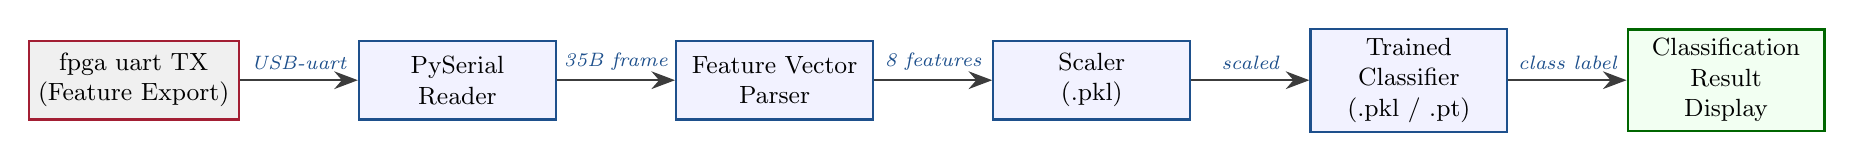
\begin{tikzpicture}[
				node distance=1.2cm and 1.5cm,
				hw/.style={rectangle, draw=stevens, fill=lightgray, thick,
					minimum width=2.5cm, minimum height=1cm, align=center, font=\small},
				sw/.style={rectangle, draw=accentblue, fill=blue!5, thick,
					minimum width=2.5cm, minimum height=1cm, align=center, font=\small},
				result/.style={rectangle, draw=green!40!black, fill=green!5, thick,
					minimum width=2.5cm, minimum height=1cm, align=center, font=\small},
				arrow/.style={-{Stealth[length=3mm]}, thick, color=darkgray},
				elabel/.style={font=\scriptsize\itshape, color=accentblue}
				]
				\node[hw] (fpga) {\FPGA{} \UART{} TX\\(Feature Export)};
				\node[sw, right=of fpga] (serial) {PySerial\\Reader};
				\node[sw, right=of serial] (parse) {Feature Vector\\Parser};
				\node[sw, right=of parse] (scale) {Scaler\\(.pkl)};
				\node[sw, right=of scale] (model) {Trained\\Classifier\\(.pkl / .pt)};
				\node[result, right=of model] (display) {Classification\\Result\\Display};

				\draw[arrow] (fpga) -- (serial) node[midway, above, elabel] {USB-\UART{}};
				\draw[arrow] (serial) -- (parse) node[midway, above, elabel] {35B frame};
				\draw[arrow] (parse) -- (scale) node[midway, above, elabel] {8 features};
				\draw[arrow] (scale) -- (model) node[midway, above, elabel] {scaled};
				\draw[arrow] (model) -- (display) node[midway, above, elabel] {class label};
			\end{tikzpicture}%
		}
		\caption{Real-time inference pipeline. The script receives feature vectors from the \FPGA{} via USB-\UART{}, applies the same preprocessing (scaling) used during training, runs the classifier, and displays the result. The scaler and model are loaded from serialized files produced during Sessions~13--15.}
		\label{fig:inference}
	\end{figure}

	\subsubsection{Real-Time Constraint}

	The inference script must classify each feature vector before the next one arrives. The inter-arrival time depends on the cooperative-target initiator cadence (Target~A's DATA schedule):

	\begin{equation}
		T_{\text{available}} = T_{\text{beacon interval}} - L_{\text{\UART{}}} = T_{\text{beacon}} - 3.73\text{~ms}
		\label{eq:realtime}
	\end{equation}

	For the minimum initiator interval tested (1~second at SF7), $T_{\text{available}} \approx 996$~ms. The inference latency budget is:

	\begin{table}[ht!]
		\centering
		\caption{Inference latency budget.}
		\label{tab:inference_latency}
		\renewcommand{\arraystretch}{1.3}
		\begin{tabularx}{\textwidth}{l c X}
			\toprule
			\textbf{Component} & \textbf{Expected} & \textbf{Notes} \\
			\midrule
			\UART{} frame reception & 3.04~ms & 35 bytes $\times$ 10 bits $\div$ 115200 baud \\
			Feature parsing & $<$0.1~ms & Python struct unpacking (includes \texttt{pkt\_type} bit-field extraction from \texttt{Modulation Code} byte if not already split by the FPGA) \\
			Scaler transform & $<$0.1~ms & Vectorized NumPy operation \\
			Random Forest inference $\times$ 4 & $<$2~ms & scikit-learn predict on 1 sample, run sequentially for SF / mod / emitter / packet-type \\
			MLP inference $\times$ 4 (alternative) & $<$2~ms & PyTorch forward pass (CPU), four task-specific models \\
			Display update & $<$1~ms & Console print or GUI update with all four predicted labels \\
			\midrule
			\textbf{Total} & $<$\textbf{8~ms} & Well within the 996~ms budget \\
			\bottomrule
		\end{tabularx}
	\end{table}

	\begin{tcolorbox}[infobox={Design Principle: Real-Time is Relative}]
		The 996~ms budget makes ``real-time'' classification trivially achievable on a modern PC. This is by design: the framework's goal is to demonstrate the complete pipeline, not to push inference speed to its limits. In a production system, the latency-critical path would be the \FPGA{} processing (6 clock cycles at 100~MHz = 60~ns), not the host-side Python inference. Students should recognize that the real-time constraint here is soft and generous, and that a production deployment would either run inference on the \FPGA{} itself (using a hardware neural network accelerator) or on an embedded processor with tighter latency requirements. Module~5 explores these architectural alternatives.
	\end{tcolorbox}

	\subsection{Inference Script Implementation}

	The inference script (\texttt{inference.py}) reuses the feature vector reception code from the Module~3 collection script but replaces the CSV writer with a classification pipeline.

	\subsubsection{Key Components}

	\begin{enumerate}[leftmargin=2em]
		\item \textbf{Model Loading:} Load the trained classifier (scikit-learn \texttt{.pkl} or PyTorch \texttt{.pt}) and the fitted scaler (\texttt{.pkl}) at startup. For PyTorch models, set the model to evaluation mode (\texttt{model.eval()}) and disable gradient computation (\texttt{torch.no\_grad()}).

		\item \textbf{Feature Reception:} Receive the 35-byte feature export frame from the \FPGA{} \UART{} TX (Module~3 Table~5), verify \CRC{}-8, extract the 32-byte feature vector, and parse it into the 8-element feature array using the same decoding logic from \texttt{preprocess.py}.

		\item \textbf{Classification:} Apply the scaler transform, run the classifier's predict method, and extract the predicted class label and (if available) the prediction probability.

		\item \textbf{Display:} Print the classification result to the console in a structured format showing all four predicted labels:
		\begin{center}
			\small\ttfamily
			[12:34:56.789] Beacon 0x01 | RSSI: -62 dBm | SNR: 8.5 dB | Pred: SF7 / LoRa / Target~A / DATA (conf: 0.94/0.99/0.91/0.88)
		\end{center}
	\end{enumerate}

	\subsubsection{Multi-Task Inference}

	The script should support running all four classification tasks simultaneously. Each received feature vector is classified for SF, modulation, emitter ID, and packet type in a single pass:

	\begin{figure}[ht!]
		\centering
		\resizebox{0.9\textwidth}{!}{%
			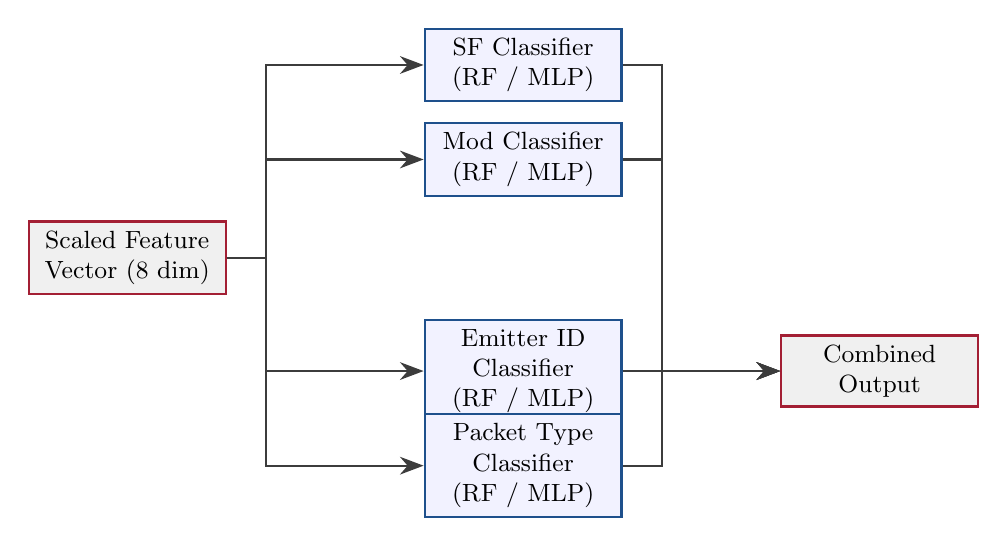
\begin{tikzpicture}[
				node distance=1.2cm and 1.5cm,
				block/.style={rectangle, draw=stevens, fill=lightgray, thick,
					minimum width=2.5cm, minimum height=0.9cm, align=center, font=\small},
				model/.style={rectangle, draw=accentblue, fill=blue!5, thick,
					minimum width=2.5cm, minimum height=0.9cm, align=center, font=\small},
				arrow/.style={-{Stealth[length=3mm]}, thick, color=darkgray},
				elabel/.style={font=\scriptsize\itshape, color=accentblue}
				]
				\node[block] (input) {Scaled Feature\\Vector (8 dim)};
				\node[model, above right=1.5cm and 2.5cm of input] (sf) {SF Classifier\\(RF / MLP)};
				\node[model, above right=0.3cm and 2.5cm of input] (mod) {Mod Classifier\\(RF / MLP)};
				\node[model, below right=0.3cm and 2.5cm of input] (eid) {Emitter ID\\Classifier\\(RF / MLP)};
				\node[model, below right=1.5cm and 2.5cm of input] (pkt) {Packet Type\\Classifier\\(RF / MLP)};

				\node[block, right=2cm of eid] (out) {Combined\\Output};

				\draw[arrow] (input.east) -- ++(0.5,0) |- (sf.west);
				\draw[arrow] (input.east) -- ++(0.5,0) |- (mod.west);
				\draw[arrow] (input.east) -- ++(0.5,0) |- (eid.west);
				\draw[arrow] (input.east) -- ++(0.5,0) |- (pkt.west);
				\draw[arrow] (sf.east) -- ++(0.5,0) |- (out.west);
				\draw[arrow] (mod.east) -- ++(0.5,0) |- (out.west);
				\draw[arrow] (eid.east) -- ++(0.5,0) |- (out.west);
				\draw[arrow] (pkt.east) -- ++(0.5,0) |- (out.west);
			\end{tikzpicture}%
		}
		\caption{Multi-task inference. A single feature vector is classified by four independent models. Each model uses the task-specific feature subset defined in Table~\ref{tab:feature_selection}, with strict adherence to the forbidden-column rules to prevent label leakage (especially for the packet-type task, where \texttt{pkt\_type} itself is the canonical leakage trap).}
		\label{fig:multi_task}
	\end{figure}

	\subsection{Live Demonstration Protocol}

	\begin{tcolorbox}[infobox={Exercise: End-to-End Live Classification}]
		With the full system running (Target~A + Target~B in ping-pong, Threat capturing and connected to the \FPGA{}, host PC):
		\begin{enumerate}
			\item Start the inference script connected to the \FPGA{}'s USB-\UART{} port.
			\item Observe real-time classification output for 60 seconds. Verify:
			\begin{itemize}
				\item SF predictions match the targets' configured spreading factor.
				\item Modulation predictions correctly identify LoRa.
				\item Emitter ID predictions distinguish between Target~A (Beacon~ID \texttt{0x01}) and Target~B (Beacon~ID \texttt{0x02}).
				\item Packet-type predictions correctly identify DATA rows from Target~A and ACK rows from Target~B.
			\end{itemize}
			\item Change Target~A's spreading factor from SF7 to SF10 (requires firmware reflash or runtime reconfiguration). Observe the inference output transition for both the SF and packet-type predictions (the slower SF10 cadence will change the inter-arrival pattern that the packet-type classifier uses).
			\item Move Target~B from 3~m to 8~m distance. Observe whether classification accuracy degrades and whether \RSSI{} changes are reflected in the console output.
			\item Hold the Threat's user button for 5~s. Verify that:
			\begin{itemize}
				\item PAUSE rows (Beacon~ID \texttt{0xFF}) appear in the inference output, classified with \texttt{pkt\_type} = PAUSE.
				\item During the button-hold window, Target~A's DATA TX stops appearing in the live stream (because Target~A is paused), and the inference output reflects this gap.
				\item After the button is released, normal DATA / ACK ping-pong resumes within $\sim$500\,ms.
			\end{itemize}
		\end{enumerate}
		\textbf{Milestone:} This demonstration represents the complete end-to-end pipeline: a physical \RF{} signal exchange between two cooperative targets, intercepted by the Threat, processed by the \FPGA{}, and classified by four parallel machine learning models, with the closed-loop intercept-and-act behavior of the PAUSE protocol observable in the live classification stream---all operating in real time.
	\end{tcolorbox}

	\subsection{Inference Latency Measurement}

	Measure the actual inference latency by timestamping each stage of the pipeline:

	\begin{enumerate}[leftmargin=2em]
		\item Record \texttt{time.perf\_counter()} immediately after \UART{} frame reception.
		\item Record \texttt{time.perf\_counter()} immediately after classification.
		\item The difference is the inference processing time (excluding \UART{} reception).
	\end{enumerate}

	Collect latency measurements for 200 consecutive classifications and report the mean, standard deviation, and 99th percentile. Verify that the 99th percentile is well below $T_{\text{available}}$.

	\subsection{Final Model Selection}

	Based on the complete results from Sessions~14--16, select the final model for each task. The selection criteria should balance:

	\begin{table}[ht!]
		\centering
		\caption{Model selection criteria.}
		\label{tab:selection}
		\renewcommand{\arraystretch}{1.3}
		\begin{tabularx}{\textwidth}{l c X}
			\toprule
			\textbf{Criterion} & \textbf{Weight} & \textbf{Justification} \\
			\midrule
			Test Accuracy / Macro F1 & 40\% & Primary performance metric. \\
			Robustness across \SNR{} range & 25\% & Model should degrade gracefully, not catastrophically. \\
			Inference Latency & 15\% & Must fit within the real-time budget. \\
			Interpretability & 10\% & Feature importances aid system understanding. \\
			Complexity / Maintenance & 10\% & Simpler models are preferred if accuracy is comparable. \\
			\bottomrule
		\end{tabularx}
	\end{table}

	\begin{tcolorbox}[infobox={Expected Outcome}]
		For this dataset size ($\sim$2{,}500 samples, 8 features), Random Forest is likely to be the best overall choice for the SF / modulation / emitter ID tasks: it typically matches or exceeds the neural network models on tabular data at this scale, provides feature importances, requires no scaling, and has negligible inference latency. The MLP may slightly outperform on tasks with complex feature interactions, while the CNN-1D is unlikely to improve over the MLP unless it operates on the windowed 8-row sequence variant (where it can exploit short-term temporal patterns in the inter-arrival sequence). The packet-type classification task is the most likely to favor the CNN-1D over the Random Forest because the discriminative signal lives in the sequential pattern of inter-arrival times across consecutive packets, not in any single row's features. The primary value of the neural network experiments is pedagogical: students learn to implement, train, and evaluate them, compare them against simpler alternatives, and make an evidence-based model selection rather than defaulting to ``deep learning is always better.''
	\end{tcolorbox}

	\begin{tcolorbox}[deliverable={Session 16 Deliverable}]
		\textbf{Real-Time Inference and Final Pipeline Report} --- A document containing:
		\begin{enumerate}
			\item Inference script source code (\texttt{inference.py}) with documentation.
			\item Live demonstration results: classification output log for the 60-second run, including the SF change and distance change experiments.
			\item Inference latency analysis: histogram of processing times, mean/std/99th percentile, comparison against real-time budget.
			\item Final model selection table: all classifiers $\times$ all four tasks, with accuracy, macro F1, robustness rating, latency, and final selection with justification.
			\item Complete \ML{} pipeline documentation: end-to-end flow from CSV to real-time classification (including the bit-field decoding of \texttt{Modulation Code}), all four task models, all file paths, dependencies, and execution instructions.
			\item Serialized model files (\texttt{.pkl} / \texttt{.pt}) for all four tasks plus the shared scaler file, ready for Module~5 system validation.
		\end{enumerate}
	\end{tcolorbox}

	\newpage
	% ══════════════════════════════════════════════════════════════
	\section{Complete Classification Pipeline Architecture}
	% ══════════════════════════════════════════════════════════════

	Figure~\ref{fig:full_ml_pipeline} shows the complete \ML{} pipeline as developed across Module~4, from data ingestion to real-time inference.

	\begin{figure}[ht!]
		\centering
		\resizebox{\textwidth}{!}{%
			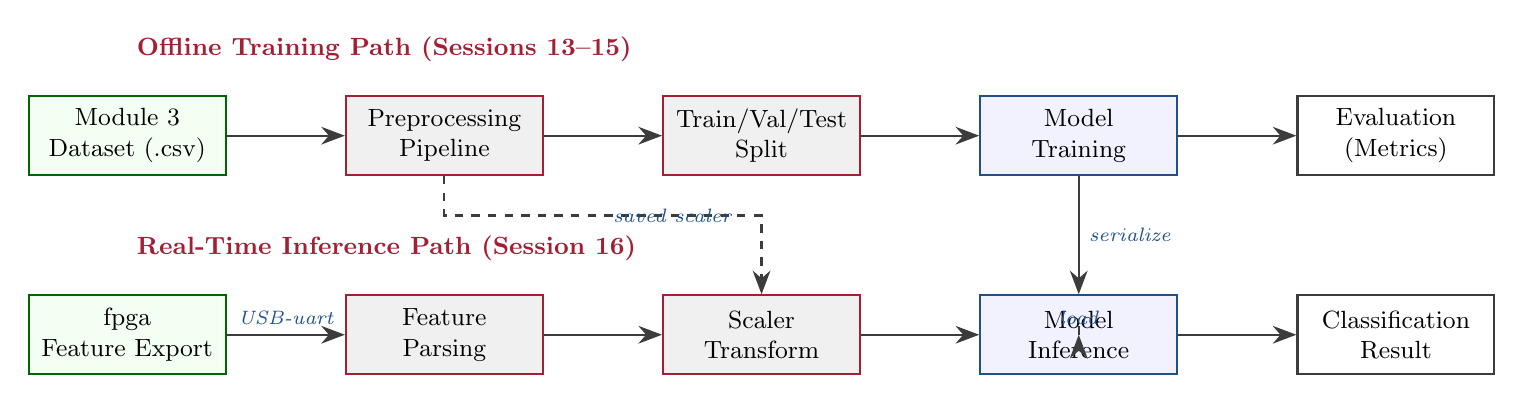
\begin{tikzpicture}[
				node distance=1cm and 1.5cm,
				data/.style={rectangle, draw=green!40!black, fill=green!5, thick,
					minimum width=2.5cm, minimum height=1cm, align=center, font=\small},
				proc/.style={rectangle, draw=stevens, fill=lightgray, thick,
					minimum width=2.5cm, minimum height=1cm, align=center, font=\small},
				model/.style={rectangle, draw=accentblue, fill=blue!5, thick,
					minimum width=2.5cm, minimum height=1cm, align=center, font=\small},
				eval/.style={rectangle, draw=darkgray, fill=white, thick,
					minimum width=2.5cm, minimum height=1cm, align=center, font=\small},
				arrow/.style={-{Stealth[length=3mm]}, thick, color=darkgray},
				elabel/.style={font=\scriptsize\itshape, color=accentblue}
				]

				% Top row: offline training path
				\node[data] (csv) {Module~3\\Dataset (.csv)};
				\node[proc, right=of csv] (preproc) {Preprocessing\\Pipeline};
				\node[proc, right=of preproc] (split) {Train/Val/Test\\Split};
				\node[model, right=of split] (train) {Model\\Training};
				\node[eval, right=of train] (eval) {Evaluation\\(Metrics)};
				\node[model, below=1.5cm of train] (saved) {Saved Model\\(.pkl / .pt)};

				% Bottom row: real-time inference path
				\node[data, below=1.5cm of csv] (fpga) {\FPGA{}\\Feature Export};
				\node[proc, right=of fpga] (parse) {Feature\\Parsing};
				\node[proc, right=of parse] (scale_rt) {Scaler\\Transform};
				\node[model, right=of scale_rt] (infer) {Model\\Inference};
				\node[eval, right=of infer] (result) {Classification\\Result};

				% Arrows - training path
				\draw[arrow] (csv) -- (preproc);
				\draw[arrow] (preproc) -- (split);
				\draw[arrow] (split) -- (train);
				\draw[arrow] (train) -- (eval);
				\draw[arrow] (train) -- (saved) node[midway, right, elabel] {serialize};

				% Arrows - inference path
				\draw[arrow] (fpga) -- (parse) node[midway, above, elabel] {USB-\UART{}};
				\draw[arrow] (parse) -- (scale_rt);
				\draw[arrow] (scale_rt) -- (infer);
				\draw[arrow] (infer) -- (result);

				% Training to inference connections
				\draw[arrow, dashed] (saved) -- (infer) node[midway, above, elabel] {load};
				\draw[arrow, dashed] (preproc.south) -- ++(0,-0.5) -| (scale_rt.north) node[near start, right, elabel] {saved scaler};

				% Labels
				\node[font=\small\bfseries\color{stevens}, above=0.3cm of csv, anchor=south west] {Offline Training Path (Sessions 13--15)};
				\node[font=\small\bfseries\color{stevens}, above=0.3cm of fpga, anchor=south west] {Real-Time Inference Path (Session 16)};
			\end{tikzpicture}%
		}
		\caption{Complete Module~4 \ML{} pipeline. The offline path (top) trains and evaluates classifiers on the Module~3 dataset. The real-time path (bottom) deploys the trained model to classify live \FPGA{} feature exports. The scaler and model artifacts connect the two paths.}
		\label{fig:full_ml_pipeline}
	\end{figure}

	\newpage
	% ══════════════════════════════════════════════════════════════
	\section{Software Reference}
	\label{sec:software}
	% ══════════════════════════════════════════════════════════════

	\begin{table}[ht!]
		\centering
		\caption{Required software and libraries for Module 4.}
		\label{tab:software}
		\renewcommand{\arraystretch}{1.3}
		\begin{tabularx}{\textwidth}{l l X}
			\toprule
			\textbf{Package} & \textbf{Version} & \textbf{Purpose} \\
			\midrule
			Python & 3.10+ & Runtime environment \\
			\texttt{pandas} & $\geq$2.0 & Dataset loading, manipulation, and CSV I/O \\
			\texttt{numpy} & $\geq$1.24 & Numerical operations, array manipulation \\
			\texttt{scikit-learn} & $\geq$1.3 & Classical classifiers (RF, SVM), metrics, preprocessing \\
			\texttt{matplotlib} & $\geq$3.7 & Plotting (confusion matrices, learning curves, bar charts) \\
			\texttt{seaborn} & $\geq$0.12 & Statistical visualizations (heatmaps, violin plots) \\
			\texttt{torch} (PyTorch) & $\geq$2.0 & Neural network models (MLP, CNN-1D) \\
			\texttt{pyserial} & $\geq$3.5 & Real-time \UART{} communication with \FPGA{} \\
			\texttt{joblib} & $\geq$1.3 & Model and scaler serialization (.pkl files) \\
			Terminal Emulator & --- & \UART{} monitoring (PuTTY, Tera Term) \\
			\bottomrule
		\end{tabularx}
	\end{table}

	\subsection{Hardware Requirements}

	\begin{table}[ht!]
		\centering
		\caption{Hardware required for Module 4.}
		\label{tab:hardware}
		\renewcommand{\arraystretch}{1.3}
		\begin{tabularx}{\textwidth}{l l X}
			\toprule
			\textbf{Item} & \textbf{Qty} & \textbf{Purpose} \\
			\midrule
			STM32 Nucleo-L476RG + RFM95W & 2 & Cooperative targets (Target~A, Target~B) for live ping-pong demonstration \\
			STM32 Nucleo-L476RG + RFM95W & 1 & Interceptor (Threat) MCU; user button (B1) reachable for PAUSE-burst demonstration \\
			Digilent Nexys A7-100T & 1 & \FPGA{} running Module~2 pipeline \\
			USB Micro-B Cables & 4--5 & Power, programming, \UART{} \\
			Host PC (any OS) & 1 & Python runtime, model training, inference \\
			\bottomrule
		\end{tabularx}
	\end{table}

	% ══════════════════════════════════════════════════════════════
	\section{Assessment Rubric}
	% ══════════════════════════════════════════════════════════════

	\begin{table}[ht!]
		\centering
		\caption{Module 4 assessment rubric.}
		\label{tab:rubric}
		\renewcommand{\arraystretch}{1.3}
		\begin{tabularx}{\textwidth}{X c c}
			\toprule
			\textbf{Assessment Item} & \textbf{Weight} & \textbf{Due} \\
			\midrule
			Data Preprocessing Report (validation, sentinels, decoding, four-task feature selection with leakage analysis, pipeline code) & 15\% & Session 13 \\
			Classical Classifier Report (baselines, RF, SVM, tuning, confusion matrices, feature importances for all four tasks) & 25\% & Session 14 \\
			Neural Network and Operating-Condition Shift Report (MLP, CNN-1D, clean$\to$contended gap on hardware data, fine-tuning recovery, performance-vs.-condition) & 30\% & Session 15 \\
			Real-Time Multi-Task Inference and Final Pipeline Report (four-task inference script, live ping-pong + PAUSE demo, latency, model selection) & 30\% & Session 16 \\
			\bottomrule
		\end{tabularx}
	\end{table}

	\newpage
	% ══════════════════════════════════════════════════════════════
	\section{Recommended Resources}
	% ══════════════════════════════════════════════════════════════

	\subsection{Machine Learning Textbooks}

	\begin{enumerate}[leftmargin=2em]
		\item A.\ G\'eron, \textit{Hands-On Machine Learning with Scikit-Learn, Keras, and TensorFlow}, 3rd ed., O'Reilly, 2022. (Chapters 2--3: classification pipeline, model evaluation, confusion matrices. Chapter 10: neural networks with Keras/PyTorch.)
		\item C.\ M.\ Bishop and H.\ Bishop, \textit{Deep Learning: Foundations and Concepts}, Springer, 2024. (Chapters 5--6: neural networks, backpropagation, regularization.)
		\item T.\ Hastie, R.\ Tibshirani, and J.\ Friedman, \textit{The Elements of Statistical Learning}, 2nd ed., Springer, 2009. (Chapter 15: Random Forests. Chapter 12: SVMs.)
	\end{enumerate}

	\subsection{RF and Signal Classification References}

	\begin{enumerate}[leftmargin=2em]
		\item T.\ J.\ O'Shea, T.\ Roy, and T.\ C.\ Clancy, ``Over-the-Air Deep Learning Based Radio Signal Classification,'' \textit{IEEE Journal of Selected Topics in Signal Processing}, vol.~12, no.~1, pp.~168--179, Feb.\ 2018.
		\item S.\ Rajendran \textit{et al.}, ``Deep Learning Models for Wireless Signal Classification With Distributed Low-Cost Spectrum Sensors,'' \textit{IEEE Transactions on Cognitive Communications and Networking}, vol.~4, no.~3, pp.~433--445, Sep.\ 2018.
		\item K.\ Merchant \textit{et al.}, ``Deep Learning for RF Device Fingerprinting in Cognitive Communication Networks,'' \textit{IEEE Journal of Selected Topics in Signal Processing}, vol.~12, no.~1, pp.~160--167, Feb.\ 2018.
	\end{enumerate}

	\subsection{Software Documentation}

	\begin{enumerate}[leftmargin=2em]
		\item scikit-learn User Guide. [Online]. Available: \url{https://scikit-learn.org/stable/user_guide.html} (Classification, model evaluation, preprocessing, pipelines.)
		\item PyTorch Tutorials. [Online]. Available: \url{https://pytorch.org/tutorials/} (Neural network training, data loading, model serialization.)
		\item pandas Documentation. [Online]. Available: \url{https://pandas.pydata.org/docs/} (DataFrame operations, CSV I/O, data cleaning.)
		\item matplotlib Gallery. [Online]. Available: \url{https://matplotlib.org/stable/gallery/} (Confusion matrix plotting, bar charts, learning curves.)
	\end{enumerate}

	\subsection{Distribution Shift and Operating-Condition Generalization}

	\begin{enumerate}[leftmargin=2em]
		\item J.\ Quinonero-Candela \textit{et al.}, \textit{Dataset Shift in Machine Learning}, MIT Press, 2009. (Foundational treatment of covariate shift, prior probability shift, and concept drift; the LH4-F operating-condition shift experiment is a covariate-shift study within the same hardware platform.)
		\item K.\ Weiss, T.\ M.\ Khoshgoftaar, and D.\ Wang, ``A Survey of Transfer Learning,'' \textit{Journal of Big Data}, vol.~3, no.~9, 2016. (Background for the freeze-and-fine-tune mitigation strategy used in LH4-F.)
	\end{enumerate}

	\newpage
	% ══════════════════════════════════════════════════════════════
	\section{Transition to Module 5}
	% ══════════════════════════════════════════════════════════════

	Upon successful completion of Module~4, students will have:
	\begin{itemize}[leftmargin=2em]
		\item A reproducible preprocessing pipeline that transforms raw \FPGA{} feature vectors into classifier-ready input, with explicit handling of sentinels, signed fields, four-task feature selection (with strict label-leakage discipline including the \texttt{pkt\_type} trap), and scaling.
		\item Trained and evaluated classifiers for four distinct tasks (spreading factor detection, modulation classification, emitter identification, packet-type classification across DATA / ACK / PAUSE) using both classical \ML{} (Random Forest, SVM) and neural network (MLP, CNN-1D) approaches.
		\item Quantitative evidence of the operating-condition distribution shift, measured through clean$\to$contended accuracy degradation entirely on hardware data, with fine-tuning recovery on the SF detection task.
		\item Performance-vs.-condition curves that characterize classifier accuracy as a function of \SNR{}, physical distance, and active-station count (across the C5a--C5e sub-configurations including PAUSE-burst scenarios), defining the system's operational classification envelope.
		\item A real-time multi-task inference script that classifies live \FPGA{} feature exports across all four tasks simultaneously, demonstrating end-to-end pipeline operation from cooperative-target \RF{} transmission, through interceptor (Threat) capture, to classification output --- including live observation of the closed-loop PAUSE intercept-and-act behavior.
		\item Serialized model and scaler artifacts (four task models + shared scaler) ready for deployment and benchmarking.
	\end{itemize}

	Module~5 will subject the complete system to stress testing and final validation. The trained classifiers from this module will be evaluated under adversarial conditions: concurrent multi-station operation at maximum density, rapid parameter changes, edge-of-range deployments, sustained PAUSE bursts, and extended-duration stability tests. The performance-vs.-condition analysis from Session~15 provides the baseline expectations; Module~5 will determine whether the system meets those expectations under sustained operational load. The closed-loop PAUSE protocol additionally provides Module~5 with two new measurement axes (response latency and RSSI-targeting accuracy) that further characterize the system's intercept-and-act behavior. The final project report and presentation will synthesize results from all five modules into a coherent narrative of cross-domain system design, integration, and evaluation.

	\vfill
	\clearpage
	\printnoidxglossary[type=\acronymtype,title={Glossary}]

	\begin{center}
		\rule{0.5\textwidth}{0.4pt}\\[6pt]
		{\small\textcolor{darkgray}{End of Module 4 Lesson Plan}}
	\end{center}

\end{document}
